\documentclass[]{scrartcl}\usepackage[]{graphicx}\usepackage[]{color}
%% maxwidth is the original width if it is less than linewidth
%% otherwise use linewidth (to make sure the graphics do not exceed the margin)
\makeatletter
\def\maxwidth{ %
  \ifdim\Gin@nat@width>\linewidth
    \linewidth
  \else
    \Gin@nat@width
  \fi
}
\makeatother

\definecolor{fgcolor}{rgb}{0.345, 0.345, 0.345}
\newcommand{\hlnum}[1]{\textcolor[rgb]{0.686,0.059,0.569}{#1}}%
\newcommand{\hlstr}[1]{\textcolor[rgb]{0.192,0.494,0.8}{#1}}%
\newcommand{\hlcom}[1]{\textcolor[rgb]{0.678,0.584,0.686}{\textit{#1}}}%
\newcommand{\hlopt}[1]{\textcolor[rgb]{0,0,0}{#1}}%
\newcommand{\hlstd}[1]{\textcolor[rgb]{0.345,0.345,0.345}{#1}}%
\newcommand{\hlkwa}[1]{\textcolor[rgb]{0.161,0.373,0.58}{\textbf{#1}}}%
\newcommand{\hlkwb}[1]{\textcolor[rgb]{0.69,0.353,0.396}{#1}}%
\newcommand{\hlkwc}[1]{\textcolor[rgb]{0.333,0.667,0.333}{#1}}%
\newcommand{\hlkwd}[1]{\textcolor[rgb]{0.737,0.353,0.396}{\textbf{#1}}}%
\let\hlipl\hlkwb

\usepackage{framed}
\makeatletter
\newenvironment{kframe}{%
 \def\at@end@of@kframe{}%
 \ifinner\ifhmode%
  \def\at@end@of@kframe{\end{minipage}}%
  \begin{minipage}{\columnwidth}%
 \fi\fi%
 \def\FrameCommand##1{\hskip\@totalleftmargin \hskip-\fboxsep
 \colorbox{shadecolor}{##1}\hskip-\fboxsep
     % There is no \\@totalrightmargin, so:
     \hskip-\linewidth \hskip-\@totalleftmargin \hskip\columnwidth}%
 \MakeFramed {\advance\hsize-\width
   \@totalleftmargin\z@ \linewidth\hsize
   \@setminipage}}%
 {\par\unskip\endMakeFramed%
 \at@end@of@kframe}
\makeatother

\definecolor{shadecolor}{rgb}{.97, .97, .97}
\definecolor{messagecolor}{rgb}{0, 0, 0}
\definecolor{warningcolor}{rgb}{1, 0, 1}
\definecolor{errorcolor}{rgb}{1, 0, 0}
\newenvironment{knitrout}{}{} % an empty environment to be redefined in TeX

\usepackage{alltt}
\usepackage[square,numbers]{natbib}
\usepackage[]{fullpage}
\usepackage{setspace}
% \doublespacing
% \VignetteIndexEntry{The surrosurv package, use and examples}
% \VignetteKeyword{Surrogate endpoints}
% \VignetteEngine{knitr::knitr}

\usepackage{listings}
\usepackage{graphicx, color, doi, xcolor, graphicx, color, amsmath, amssymb, bm, hyperref, textcomp, thumbpdf}
\usepackage{lineno}

%%%%%%%%%%%%%%%%%%%%%%%%%%%%%%
%% declarations for jss.cls %%%%%%%%%%%%%%%%%%%%%%%%%%%%%%%%%%%%%%%%%%
%%%%%%%%%%%%%%%%%%%%%%%%%%%%%%
\IfFileExists{upquote.sty}{\usepackage{upquote}}{}
\begin{document}
\definecolor{darkgray}{rgb}{.15, .12, .11}
\lstset{ %
  language=R,                     % the language of the code
  upquote=true,
  basicstyle=\small\ttfamily\color{darkgray},       % the size of the fonts that are used for the code
  numbers=left,                   % where to put the line-numbers
  numberstyle=\tiny\color{darkgray},  % the style that is used for the line-numbers
  stepnumber=5,                   % the step between two line-numbers. If it's 1, each line
                                  % will be numbered
  numbersep=5pt,                  % how far the line-numbers are from the code
  backgroundcolor=\color{white},  % choose the background color. You must add \usepackage{color}
  showspaces=false,               % show spaces adding particular underscores
  showstringspaces=false,         % underline spaces within strings
  showtabs=false,                 % show tabs within strings adding particular underscores
  % frame=single,                   % adds a frame around the code
  rulecolor=\color{black},        % if not set, the frame-color may be changed on line-breaks within not-black text (e.g. commens (green here))
  tabsize=2,                      % sets default tabsize to 2 spaces
  captionpos=b,                   % sets the caption-position to bottom
  breaklines=true,                % sets automatic line breaking
  breakatwhitespace=false,        % sets if automatic breaks should only happen at whitespace
  title=\lstname,                 % show the filename of files included with \lstinputlisting;
                                  % also try caption instead of title
  % keywordstyle=\color{blue},      % keyword style
  commentstyle=\color{dkgreen},   % comment style
  stringstyle=\color{brown},      % string literal style
  escapeinside={\%*}{*)},         % if you want to add a comment within your code
  morekeywords={*,...}            % if you want to add more keywords to the set
}
\def\inline{\lstinline[basicstyle=\ttfamily\color{darkgray}]}


\author{Federico Rotolo$^{1, 2,}$\footnote{
  114, Rue Edouard Vaillant -- Villejuif, F-94805, France.
  \href{mailto:federico.rotolo@gustaveroussy.fr}{federico.rotolo@gustaveroussy.fr}.
  +33~1~42~11~61~28},
  Xavier Paoletti$^{1, 2}$, Stefan Michiels$^{1, 2}$}
\date{\footnotesize{$^1$ Service de Biostatistique et d'\'Epid\'emiologie, Gustave Roussy\\
      $^2$ INSERM U1018 OncoStat, CESP}}

\title{\inline{surrosurv}:
      an \inline{R} Package for the Evaluation of Failure Time Surrogate Endpoints
      in Individual Patient Data Meta-Analyses of Randomized Clinical Trials}

% \maketitle

%%%%%%%%%%%%%%%%%%%%%%%%%%%%%%%%%%%%%%%%%%%%%%%%%%%%%%%%%%%%%%%%%%%%%%%%%%%%%%%%
%%%%%%%%%%%%%%%%%%%%%%%%%%%%%%%%%%%%%%%%%%%%%%%%%%%%%%%%%%%%%%%%%%%%%%%%%%%%%%%%
%%%%%%%%%%%%%%%%%%%%%%%%%%%%%%%%%%%%%%%%%%%%%%%%%%%%%%%%%%%%%%%%%%%%%%%%%%%%%%%%
\subsection*{%Title}
\inline{surrosurv}:
an \inline{R} Package for the Evaluation of Failure Time Surrogate Endpoints
in Individual Patient Data Meta-Analyses of Randomized Clinical Trials
}
% \subsection*{Authors}
Federico Rotolo$^{1, 2}$ %\newline
Xavier Paoletti$^{1, 2}$ %\newline
Stefan Michiels$^{1, 2}$

% \subsection*{Affiliations}
$^1$ Service de Biostatistique et d'\'Epid\'emiologie, Gustave Roussy, Univ. Paris-Saclay
\newline
$^2$ INSERM U1018 OncoStat, CESP, Univ. Paris-Sud, Univ. Paris-Saclay

% \subsection*{Full contact of the corresponding author}
% Federico Rotolo, PhD\newline
% Service de Biostatistique et d'\'Epid\'emiologie\newline
% Gustave Roussy Cancer Campus\newline
% 114, Rue Edouard Vaillant -- Villejuif, CEDEX\newline
% F-94805, France.\newline
% \href{mailto:federico.rotolo@gustaveroussy.fr}{federico.rotolo@gustaveroussy.fr}
% \newline
% +33~1~42~11~61~28
%     
% \subsection*{Target journal}
% Computer Methods and Programs in Biomedicine\newline
% Section II. Systems and Programs.
%%%%%%%%%%%%%%%%%%%%%%%%%%%%%%%%%%%%%%%%%%%%%%%%%%%%%%%%%%%%%%%%%%%%%%%%%%%%%%%%
%%%%%%%%%%%%%%%%%%%%%%%%%%%%%%%%%%%%%%%%%%%%%%%%%%%%%%%%%%%%%%%%%%%%%%%%%%%%%%%%
%%%%%%%%%%%%%%%%%%%%%%%%%%%%%%%%%%%%%%%%%%%%%%%%%%%%%%%%%%%%%%%%%%%%%%%%%%%%%%%%
  
% \newpage
\onehalfspacing
\section*{Abstract}
  \paragraph{Background and Objective.}
  Surrogate endpoints are attractive for use in clinical trials
    instead of well-established endpoints because of practical convenience.
  To validate a surrogate endpoint,
    two important measures can be estimated in a meta-analytic context
    when individual patient data are available:
    the $R^2_\text{indiv}$ or the Kendall's $\tau$ at the individual level,
    and the  $R^2_\text{trial}$ at the trial level.
  We aimed at providing an \inline{R} implementation of
    classical and well-established as well as more recent statistical methods
    for surrogacy assessment with failure time endpoints.
  We also intended incorporating utilities for model checking and visualization
    and data generating methods described in the literature to date.
  % 
  \paragraph{Methods.}
  In the case of failure time endpoints,
    the classical approach is based on two steps.
  First,  a Kendall's $\tau$ is estimated as measure of individual level surrogacy
    using a copula model.
  Then, the $R^2_\text{trial}$ is computed via a linear regression of the estimated treatment effects;
    at this second step, the estimation uncertainty can be accounted for
    via measurement-error model or via weights.
  In addition to the classical approach,
    we recently developped an approach based on bivariate 
    auxiliary Poisson models with
    individual random effects to measure the Kendall's $\tau$ and
    treatment-by-trial interactions to measure the $R^2_\text{trial}$.
  The most common data simulation models described in the literature
    are based on: copula models,
    mixed proportional hazard models, and 
    mixture of half-normal and exponential random variables.
  %
  \paragraph{Results.}
  The \inline{R} package \inline{surrosurv} implements
    the classical two-step method with Clayton, Plackett, and Hougaard copulas.
  It also allows to optionally adjust the second-step linear regression 
    for measurement-error.
  The mixed Poisson approach is implemented 
    with different reduced models in addition to the full model.
  We present the package functions for estimating the surrogacy models,
    for checking their convergence, 
    for performing leave-one-trial-out cross-validation,
    and for plotting the results.
  We illustrate their use in practice
    on individual patient data from a meta-analysis of 4069 patients with advanced
    gastric cancer from 20 trials of chemotherapy.
  %
  \paragraph{Conclusions.}
  The \inline{surrosurv} package provides an \inline{R} implementation of
  classical and recent statistical methods for surrogacy assessment
    of failure time endpoints.
  Flexible simulation functions are available
    to generate data according to the methods described in the literature.
  
%   \paragraph{Keywords.}
%     surrogate endpoints;
%     survival;
%     % time-to-event;
%     % randomized clinical trials;
%     individual patient data meta-anayses;
%     \inline{R};
%     copula;
%     mixed %proportional hazard 
%       models
%     % Poisson regression
% \clearpage
% \doublespacing
\linenumbers




% \setkeys{Gin}{width=\textwidth}

%%%%%%%%%%%%%%%%%%%%%%%%%%%%%%%%%%%%%%%%%%%%%%%%%%%%%%%%%%%%%%%%%%%%%%%%%%%%%%%%
%%%%%%%%%%%%%%%%%%%%%%%%%%%%%%%%%%%%%%%%%%%%%%%%%%%%%%%%%%%%%%%%%%%%%%%%%%%%%%%%
%%%%%%%%%%%%%%%%%%%%%%%%%%%%%%%%%%%%%%%%%%%%%%%%%%%%%%%%%%%%%%%%%%%%%%%%%%%%%%%%
\section{Introduction}
%%%%%%%%%%%%%%%%%%%%%%%%%%%%%%%%%%%%%%%%%%%%%%%%%%%%%%%%%%%%%%%%%%%%%%%%%%%%%%%%
%%%%%%%%%%%%%%%%%%%%%%%%%%%%%%%%%%%%%%%%%%%%%%%%%%%%%%%%%%%%%%%%%%%%%%%%%%%%%%%%
%%%%%%%%%%%%%%%%%%%%%%%%%%%%%%%%%%%%%%%%%%%%%%%%%%%%%%%%%%%%%%%%%%%%%%%%%%%%%%%%

Surrogate endpoints are endpoints which can reliably be used
  instead of well-established (true) endpoints
  and which yield improved practical convenience
  in terms of lower cost,
  more rapid occurrence,
  increased ease of assessment, 
  or reduced invasiveness \citep{Burzykowski2006}.
Two conditions must be fulfilled for surrogate endpoint to be reliable:
  it must be strongly associatied with
  the true endpoint at the individual level and
  the effect of the treatment on it
  must be strongly assciated with the effect on the true endpoint.
In a meta-analytic context and when the endpoints are gaussian \citep{BuyseEtal00},
  the usual measure of individual level surrogacy is
  the $R^2_\text{\tiny indiv}$ between the \textit{endpoints},
  which measures the part of variability of the true endpoint $T$
  explained by the surrogate endpoint $S$.
At the trial level, the usual measure of surrogacy
  is given by the $R^2_\text{\tiny trial}$
  between the \textit{treatment effects} on the two endpoints,
  that measures the part of variability of the \textit{treatment effect} on $T$
  explained by the \textit{treatment effect} on $S$.

In the case of failure time (survival) endpoints,
  the classical methods developped for normally-distributed endpoints
  cannot be used because of right censoring.
Burzykowski and colleagues \cite{BurzykowskiEtal01} developped a meta-analytic model
  for failure time endpoints that measures
  individual level surrogacy in terms of Kendall's $\tau$ \citep{Kendall38}
  and trial level surrogacy in terms of $R^2_\text{\tiny trial}$.
This method is largely employed in numerous applications in the medical literature.
Because of some limitations including convergence issues,
  the interpretation of the results is difficult in some cases
  \citep{Oba2013, BurzykowskiCortinas05}.
Recently, we considered using bivariate mixed proportional hazard models
   \citep{DuchateauJanssen08},
  which are the most natural adaptation of the above-mentioned
  meta-analytic approach by Buyse et al.~\cite{BuyseEtal00} to the survival case.
We exploited \citep{RotoloPoissurogate}
  the connection between the proportional hazard models
  and the Poisson log-linear models \citep{Whitehead80, LairdOlivier81}
  to build the joint model for the two treatment effects adjusted
  for individual dependence and baseline heterogeneity across trials.

In the present paper, we show how the classical and more recent models
  can be fitted by use of the \inline{R} \citep{R}
  package \inline{surrosurv} \citep{R:surrosurv}.
Model checking can be performed thanks to utilities for convergence assessment
    and leave-one-trial-out crossvalidation.
User-friendly functions allow the user to clearly show the results of the 
    estimated models.
We illustrate the available functions 
  using individual data of a meta-analysis of 20 randomized trials of chemotherapy,
  including 4069 patients with advanced/recurrent gastric cancer
  \citep{GASTRIC13, Paoletti2013}.


%%%%%%%%%%%%%%%%%%%%%%%%%%%%%%%%%%%%%%%%%%%%%%%%%%%%%%%%%%%%%%%%%%%%%%%%%%%%%%%%
%%%%%%%%%%%%%%%%%%%%%%%%%%%%%%%%%%%%%%%%%%%%%%%%%%%%%%%%%%%%%%%%%%%%%%%%%%%%%%%%
%%%%%%%%%%%%%%%%%%%%%%%%%%%%%%%%%%%%%%%%%%%%%%%%%%%%%%%%%%%%%%%%%%%%%%%%%%%%%%%%
\section{Computational methods and theory}
\label{sec:methods}
%%%%%%%%%%%%%%%%%%%%%%%%%%%%%%%%%%%%%%%%%%%%%%%%%%%%%%%%%%%%%%%%%%%%%%%%%%%%%%%%
%%%%%%%%%%%%%%%%%%%%%%%%%%%%%%%%%%%%%%%%%%%%%%%%%%%%%%%%%%%%%%%%%%%%%%%%%%%%%%%%
%%%%%%%%%%%%%%%%%%%%%%%%%%%%%%%%%%%%%%%%%%%%%%%%%%%%%%%%%%%%%%%%%%%%%%%%%%%%%%%%

Let $T_{ij}$ and $S_{ij}$ be the times to the true and the surrogate 
  endpoints, respectively,
  for patient $j\in\{1, \ldots, n_i\}$
  in trial  $i\in\{1, \ldots, N\}$.
Let $Z_{ij}$ be the indicator of the treatment arm
  to which the $j$-th patient in the $i$-th trial has been randomized.


%%%%%%%%%%%%%%%%%%%%%%%%%%%%%%%%%%%%%%%%%%%%%%%%%%%%%%%%%%%%%%%%%%%%%%%%%%%%%%%%
%%%%%%%%%%%%%%%%%%%%%%%%%%%%%%%%%%%%%%%%%%%%%%%%%%%%%%%%%%%%%%%%%%%%%%%%%%%%%%%%
\subsection{Two-step copula approach}
%%%%%%%%%%%%%%%%%%%%%%%%%%%%%%%%%%%%%%%%%%%%%%%%%%%%%%%%%%%%%%%%%%%%%%%%%%%%%%%%
%%%%%%%%%%%%%%%%%%%%%%%%%%%%%%%%%%%%%%%%%%%%%%%%%%%%%%%%%%%%%%%%%%%%%%%%%%%%%%%%
\label{sec:copulaApp}
The model proposed by {Burzykowski et al.~\cite{BurzykowskiEtal01} for failure time endpoints
  consists in two steps, one for the individual and one for the trial level.

\paragraph{Individual-level.}
At the first step, the bivariate proportional hazard model is defined
  by means of the marginal hazard functions and
  of the copula function to account for their dependence:
  \begin{equation}
    \begin{cases}
      h_{Sij}(s; Z_{ij}) = h_{Si}(s) \exp\big\{
        \alpha_i Z_{ij} 
      \big\}\\
      h_{Tij}(t; Z_{ij}) = h_{Ti}(t) \exp\big\{
        \beta_i Z_{ij}
      \big\}\\
      C_\theta(S_{Sij}(s), S_{Tij}(t))
    \end{cases}
    \label{eq:copulaModel}
  \end{equation}
  where $h_{Si}(s)$ and $h_{Ti}(s)$ are the trial-specific baseline hazards,
  $\alpha_i$ and $\beta_i$ the treatment effects,
  and $S_{Sij}(s)$ and $S_{Tij}(t)$ the survival functions associated to
  $h_{Tij}$ and $h_{Tij}$.
The dependence parameter $\theta$
  is reparametrized into the individual-level Kendall's $\tau$,
  according to the copula function
  thanks to the \inline{tau()} function in the 
  \inline{copula} package \citep{R:copula, Yan07}.

In the \inline{surrosurv} package,
  Weibull marginal hazards are implemented,
  together with three copula functions:
  \begin{itemize}
    \item the Clayton copula \citep{Clayton78}
      \begin{equation}
        C_\theta(u, v)= \left(u^{-\theta} + v^{-\theta} - 1\right)^{-1/\theta},
        \label{eq:clayton}
      \end{equation}
      with $\theta > 0$
      and Kendall's $\tau = \theta/(\theta+2)$;
    \item the Plackett copula \citep{Plackett65}
      \begin{align}
        C_\theta(u,v) &= \big[ Q - R^{1/2} \big] / \big[2 (\theta - 1) \big],\\
        Q &= 1 +(\theta-1)(u+v), \nonumber\\
        R &= Q^2 - 4 \theta(\theta-1)uv, \nonumber
      \end{align}
      with $\theta > 0$ and Kendall's $\tau$ computed using numerical integration
      as no analytical expression is available;
    \item the Hougaard copula \citep{Hougaard86}
      \begin{equation}
        C_\theta(u,v) = \exp\left(-\left[(- \ln u)^{1/\theta} +
        (- \ln v)^{1/\theta}\right]^\theta \right),
      \end{equation}
      with $\theta \in (0, 1)$ 
      and Kendall's $\tau = 1 - \theta$.
  \end{itemize}
Further details on these three copula models can be found in the 
  \inline{vignette('copula', package = 'surrosurv')}.

\paragraph{Trial level.}
At the second step, the estimates of the treatment effects 
  obtained at the first step are assumed to follow the mixed model
  \begin{align}
    \left(\begin{array}{c} 
      {\hat\alpha_i}\\ {\hat\beta_i}\end{array}\right)
    &= \left(\begin{array}{c} \alpha_i\\ \beta_i\end{array}\right) +
      \left(\begin{array}{c} \epsilon_{ai}\\ \epsilon_{bi}\end{array}\right),
    \\
    \left(\begin{array}{c} {\alpha_i}\\ {\beta_i}\end{array}\right)
    & \sim \mathcal N
      \left(
      \left(\begin{array}{c}
      \alpha\\ \beta\end{array}\right), 
      \bm D = \left(\begin{array}{cc} 
      d_a^2 &
      d_a d_b{\rho_\text{\tiny trial}} \\
      d_a d_b{\rho_\text{\tiny trial}} &
      d_b^2 \\
      \end{array}\right)
      \right),
      \label{eq:trtEffs}
    \\
    \left(\begin{array}{c} \epsilon_{ai}\\ \epsilon_{bi}\end{array}\right)
    &\sim \mathcal N \left(
      \left(\begin{array}{c}0\\0\end{array}\right),
      \bm\Omega_i = \left(\begin{array}{cc} 
            \omega_{ai}^2 &
            \omega_{ai} \omega_{bi} {\rho_{\epsilon i}} \\
            \omega_{ai} \omega_{bi} {\rho_{\epsilon i}} &
            \omega_{bi}^2 \\
        \end{array}\right)\right).
  \end{align}
  where $(\alpha_i, \beta_i)^\prime$ are the true treatment effects
  and $(\epsilon_{ai}, \epsilon_{bi})^\prime$ the estimation errors.

The trial-level surrogacy measure is
  $R_\text{\tiny trial}^2 = \rho_\text{\tiny trial}^2$.
In practice, we compute the $\rho_\text{\tiny trial}$ 
  via a linear regression of the $\beta_i$'s over the $\alpha_i$'s
  adjusted by measurement error by fixing the $\bm\Omega_i$'s at their estimates
  from the first step \citep{vanHouwelingenEtal02}
  by using the \inline{mvmeta} package \citep{GasparriniEtal12, R:mvmeta}.
This adjusted (for measurement error) model is sometimes computationally challenging
  and does not always converge.
The \inline{surrosurv} package returns also the so-called
  unadjusted $R_\text{\tiny trial}^2$,
  obtained using a linear regression ---
  equivalent to fixing all the elements of $\bm\Omega_i$ equal to 0 ---
  by weigthing the observations $(\alpha_i, \beta_i)^\prime$ by the trial size,
  in order to account somehow indirectly and approximately for estimation uncertainty.



%%%%%%%%%%%%%%%%%%%%%%%%%%%%%%%%%%%%%%%%%%%%%%%%%%%%%%%%%%%%%%%%%%%%%%%%%%%%%%%%
%%%%%%%%%%%%%%%%%%%%%%%%%%%%%%%%%%%%%%%%%%%%%%%%%%%%%%%%%%%%%%%%%%%%%%%%%%%%%%%%
\subsection{One-step mixed Poisson approach}
%%%%%%%%%%%%%%%%%%%%%%%%%%%%%%%%%%%%%%%%%%%%%%%%%%%%%%%%%%%%%%%%%%%%%%%%%%%%%%%%
%%%%%%%%%%%%%%%%%%%%%%%%%%%%%%%%%%%%%%%%%%%%%%%%%%%%%%%%%%%%%%%%%%%%%%%%%%%%%%%%

Let us assume that the bivariate proportional hazard model given by the first
  two lines of equation (\ref{eq:copulaModel}) holds conditionally
  on an individual random effect
  $u_{ij} \sim \mathcal N(0, \sigma^2_\text{\tiny indiv})$:
  \begin{equation}
    \begin{cases}
      h_{Sij}(s\mid u_{ij}) = h_{S i}(s)
      \exp\left\{u_{ij} + \alpha_i Z_{ij} \right\}\\
      h_{Tij}(t\mid u_{ij}) = h_{T i}(t)
      \exp\left\{u_{ij} + \beta_i Z_{ij}\right\}.
    \end{cases}
    \label{eq:biHaz}
  \end{equation}
Note that this corresponds to a  shared frailty model with 
  bivariate clusters \citep{DuchateauJanssen08}.
The shared frailty term $u_{ij}$ accounts for individual level dependence.

It is well-known (see for instance \cite{Whitehead80, crowtherEtal12})
  that the parameters of Cox models can be estimated by fitting
  a so-called `auxiliary' Poisson log-linear regression model,
  by dividing the time scale into intervals $k=1, \ldots, K$.
The auxiliary Poisson model provides the same estimator as the Cox model
  if the bounds of the intervals are all the observed event times,
  and an approximation of the Cox estimators otherwise.
In the surrogacy assessment context,
  the parameters of the bivariate frailty model (\ref{eq:biHaz})
  can be estimated via a bivariate mixed Poisson model
  \begin{equation}
    \begin{cases}
      \log\left( \mu_{S ij}^{(k)} \right) = 
        \mu_{S i}^{(k)}  + u_{ij}
        + \alpha_i Z_{ij}
        + \log\left(y_{S ij}^{(k)} \right)\\
      \log\left( \mu_{T ij}^{(k)} \right) = 
        \mu_{T i}^{(k)}  + u_{ij}
        + \beta_i Z_{ij}
        + \log\left(y_{T ij}^{(k)} \right)
    \end{cases}
    \label{eq:biPoiMix}
  \end{equation}
  with $y_{Sj}^{(k)}$ and $y_{Tj}^{(k)}$ the time spent at risk
  by subject $i$ in trial $j$ for each endpoint
  during the period $k$.


%%%%%%%%%%%%%%%%%%%%%%%%%%%%%%%%%%%%%%%%%%%%%%%%%%%%%%
\paragraph{Individual-level surrogacy.}
%%%%%%%%%%%%%%%%%%%%%%%%%%%%%%%%%%%%%%%%%%%%%%%%%%%%%%
The estimated variance of the shared frailties $u_{ij}$
  is $\hat\sigma^2_\text{\tiny indiv}$ and 
  can be used to estimate the Kendall's
$\hat\tau = 4 \int_0^\infty s \mathcal L(s)\mathcal L^{(2)}(s) \textrm d s - 1$,
where $\mathcal L(s)$ and $\mathcal L^{(2)}(s)$
are the Laplace transform of the frailty distribution and its
second derivative.
As an analytic expression of $\mathcal L(s)$
is not available for the log-normal frailty distribution,
we approximated it using the Laplace method \citep{GoutisCasella99},
implemented in the \inline{fr.lognormal()} function
in the \inline{parfm} package \citep{parfmJSS, R:parfm}.


%%%%%%%%%%%%%%%%%%%%%%%%%%%%%%%%%%%%%%%%%%%%%%%%%%%%%%
\paragraph{Trial-level surrogacy.} \label{sec:trialDep}
%%%%%%%%%%%%%%%%%%%%%%%%%%%%%%%%%%%%%%%%%%%%%%%%%%%%%%
In model (\ref{eq:biPoiMix}),
  the trial-specific treatment effects are again assumed to follow
  the binormal distribution (\ref{eq:trtEffs}).
Thus, the correlation $\rho_\text{\tiny trial}$
  between the two treatment effects provides us with 
  the coefficient of determination
  $R^2_\text{\tiny trial} = \rho^2_\text{\tiny trial}$,
  also referred to simply as $R^2$.


%%%%%%%%%%%%%%%%%%%%%%%%%%%%%%%%%%%%%%%%%%%%%%%%%%%%%%
\paragraph{Reduced Poisson models.}
%%%%%%%%%%%%%%%%%%%%%%%%%%%%%%%%%%%%%%%%%%%%%%%%%%%%%%
The \inline{surrosurv} package can compute four reduced versions 
  of the full model (\ref{eq:biPoiMix})
  that may turn out to be useful in case of convergence issues with the full model.
\begin{itemize}
\item Model \textbf{Poisson T} has
  random trial-treatment interactions $\alpha_i$ and $\beta_i$,
  but does not incorporate individual effects ($u_{ij} \equiv 0$).
It assumes common baselines between trials
($\mu^{(k)}_{Si} = \mu^{(k)}_{S}$, $\mu^{(k)}_{Ti} = \mu^{(k)}_{T},
\forall i$).
This model provides only the trial-level measure of surrogacy
$R^2_{\textsf{\tiny trial}}$.

\item Model \textbf{Poisson I} contains individual random effects $u_{ij}$,
but not the trial-specific treatment effects 
($\alpha_i = \alpha$, $\beta_i = \beta, \forall i$)
and has common baselines between trials.
This model provides only the individual-level measure of surrogacy
$\tau$.

\item Model \textbf{Poisson TI} incorporates
both random trial-treatment interactions
$(\alpha_i, \beta_i)^\prime$
and individual random effects $u_{ij}$,
but still has common baselines between trials.
It provides both individual-level and trial-level measures of surrogacy
$\tau$ and $R^2_{\textsf{\tiny trial}}$.

\item Model \textbf{Poisson TIa} extends the model Poisson TI
by accounting for trial-specific baseline risks,
using shared random effects at the trial level:
$\mu_{Si} = \mu_S + m_i, \mu_{Ti} = \mu_T + m_i$,
with $m_i\sim\mathcal N(0, \sigma^2_m)$.
\end{itemize}



%%%%%%%%%%%%%%%%%%%%%%%%%%%%%%%%%%%%%%%%%%%%%%%%%%%%%%%%%%%%%%%%%%%%%%%%%%%%%%%%
%%%%%%%%%%%%%%%%%%%%%%%%%%%%%%%%%%%%%%%%%%%%%%%%%%%%%%%%%%%%%%%%%%%%%%%%%%%%%%%%
%%%%%%%%%%%%%%%%%%%%%%%%%%%%%%%%%%%%%%%%%%%%%%%%%%%%%%%%%%%%%%%%%%%%%%%%%%%%%%%%
\section{Program description with a data example}
%%%%%%%%%%%%%%%%%%%%%%%%%%%%%%%%%%%%%%%%%%%%%%%%%%%%%%%%%%%%%%%%%%%%%%%%%%%%%%%%
%%%%%%%%%%%%%%%%%%%%%%%%%%%%%%%%%%%%%%%%%%%%%%%%%%%%%%%%%%%%%%%%%%%%%%%%%%%%%%%%
%%%%%%%%%%%%%%%%%%%%%%%%%%%%%%%%%%%%%%%%%%%%%%%%%%%%%%%%%%%%%%%%%%%%%%%%%%%%%%%%
We illustrate the use of the functions in the \inline{surrosurv} package
  on the individual patient data of the advanced GASTRIC meta-analysis
\citep{GASTRIC13, Paoletti2013}.
\begin{knitrout}
\definecolor{shadecolor}{rgb}{0.969, 0.969, 0.969}\color{fgcolor}\begin{kframe}
\begin{alltt}
\hlkwd{library}\hlstd{(surrosurv)}
\end{alltt}


{\ttfamily\noindent\color{warningcolor}{\#\# Warning: package 'surrosurv' was built under R version 3.2.5}}

{\ttfamily\noindent\itshape\color{messagecolor}{\#\# Loading required package: optimx}}

{\ttfamily\noindent\color{warningcolor}{\#\# Warning: package 'optimx' was built under R version 3.2.5}}\begin{alltt}
\hlkwd{packageVersion}\hlstd{(}\hlstr{'surrosurv'}\hlstd{)}
\end{alltt}
\begin{verbatim}
## [1] '1.1.10'
\end{verbatim}
\end{kframe}
\end{knitrout}

The individual data of the 4069 patients,
  already made public by \cite{BuyseEtal15},
are also available directly in \inline{R} in the \inline{surrosurv} package:
\begin{knitrout}
\definecolor{shadecolor}{rgb}{0.969, 0.969, 0.969}\color{fgcolor}\begin{kframe}
\begin{alltt}
\hlkwd{data}\hlstd{(}\hlstr{'gastadv'}\hlstd{)}
\hlkwd{nrow}\hlstd{(gastadv)}
\end{alltt}
\begin{verbatim}
## [1] 4069
\end{verbatim}
\end{kframe}
\end{knitrout}

The data set contains the following variables:
\begin{knitrout}
\definecolor{shadecolor}{rgb}{0.969, 0.969, 0.969}\color{fgcolor}\begin{kframe}
\begin{alltt}
\hlkwd{names}\hlstd{(gastadv)}
\end{alltt}
\begin{verbatim}
## [1] "timeT"    "statusT"  "statusS"  "timeS"    "trialref" "trt"     
## [7] "id"
\end{verbatim}
\end{kframe}
\end{knitrout}
where \inline{timeT} and \inline{timeS} are the (possibly censored) times 
for overall survival (\inline{T}) and
for progression-fre survival (\inline{S}) expressed in days,
\inline{statusT} and \inline{statusS} are the associated indicators of
censoring (\inline{0}) or event (\inline{1}),
\inline{trialref} is the trial indicator ($i$),
\inline{trt} is the treatment arm (\inline{-0.5} for control and \inline{0.5} for chemotherapy),
and \inline{id} is the patient indicator ($j$).
Figure~\ref{fig:survCurves} shows the Kaplan--Meier curves for overall survival,
the true endpoint $T$, and progression-free survival,
the candiddate surrogate $S$.
\begin{knitrout}
\definecolor{shadecolor}{rgb}{0.969, 0.969, 0.969}\color{fgcolor}\begin{kframe}


{\ttfamily\noindent\color{warningcolor}{\#\# Warning: package 'survival' was built under R version 3.2.5}}\end{kframe}\begin{figure}
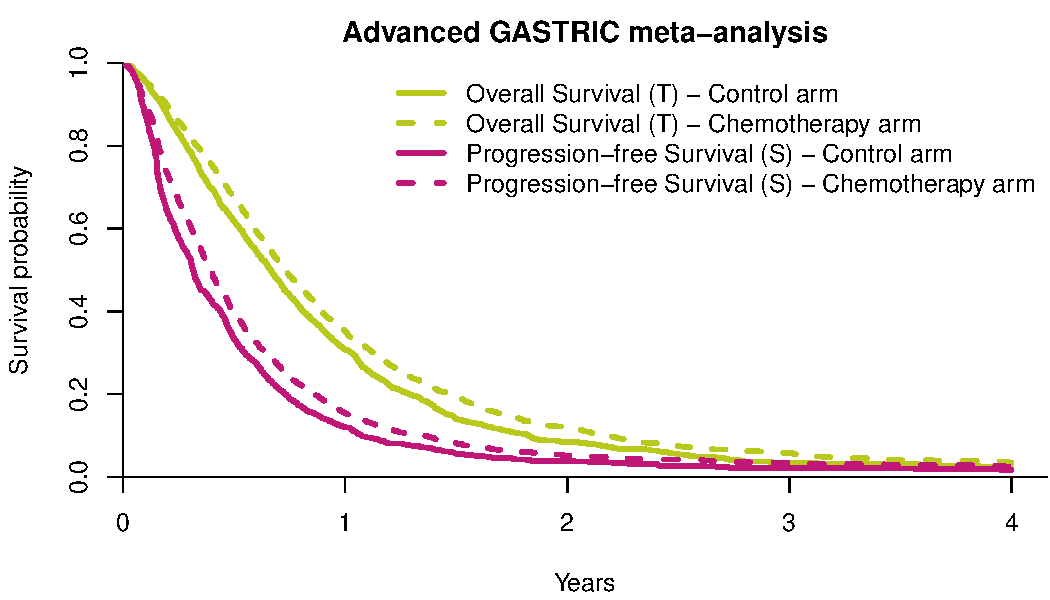
\includegraphics[width=\maxwidth]{figs/figsurvCurves-1} \caption[Survival curves for overall survival ($T$) and progression-free survival $S$ in the advanced GASTRIC meta-analysis]{Survival curves for overall survival ($T$) and progression-free survival $S$ in the advanced GASTRIC meta-analysis}\label{fig:survCurves}
\end{figure}


\end{knitrout}

  
%%%%%%%%%%%%%%%%%%%%%%%%%%%%%%%%%%%%%%%%%%%%%%%%%%%%%%%%%%%%%%%%%%%%%%%%%%%%%%%%
%%%%%%%%%%%%%%%%%%%%%%%%%%%%%%%%%%%%%%%%%%%%%%%%%%%%%%%%%%%%%%%%%%%%%%%%%%%%%%%%
\subsection{Fitting the surrogacy models}
%%%%%%%%%%%%%%%%%%%%%%%%%%%%%%%%%%%%%%%%%%%%%%%%%%%%%%%%%%%%%%%%%%%%%%%%%%%%%%%%
%%%%%%%%%%%%%%%%%%%%%%%%%%%%%%%%%%%%%%%%%%%%%%%%%%%%%%%%%%%%%%%%%%%%%%%%%%%%%%%%
  The surrogacy models presented in Section~\ref{sec:methods}
  can be fitted via the \inline{surrosurv()} function.
  
  The only mandatory argument for the \inline{surrosurv()} function is
  \inline{data}, which has to be a data.frame with columns
  \begin{itemize}
  \item \inline{trialref}, a factor containing the trial identifier;
  \item \inline{trt}, the treatment arm, coded as \inline{-0.5} \textit{vs.} \inline{0.5};
  \item \inline{id}, a factor containing the patient id;
  \item \inline{timeT} and \inline{timeS}, two positive-valued numerical variables,
  containing the observed or censored times of the true endpoint $T$
  and of the candidate surrogate $S$, respectively;
  \item \inline{statusT} and \inline{statusS},
  the censoring/event (\inline{0}/\inline{1}) indicators of $T$ and $S$, respectively.
  \end{itemize}
  
  A second argument, \inline{models}, can optionally contain the list of the models to fit
  (any of \inline{clayton}, \inline{plackett}, \inline{hougaard}, or \inline{poisson}).
  If not specified, all of them are fitted.
  
  Two further parameters, \inline{intWidth} and \inline{nInts},
  specify the width and the number of time intervals for data Poissonization.
These parameters are passed to the function \inline{poissonize()},
  described in the Appendix (Sec.~\ref{sec:poisson}).
  At most one of them can be specified.
  By default, \inline{nInts = 8} which means that the study period is divided into
  eight periods, the length of which is fixed so that 1/8th of the observed
  events falls in each interval.
  
  The optimizer used for optimization of the copula models and the Poisson models
  can be passed to the \inline{optimx} package \citep{optimxJSS, R:optimx}
  via the arguments \inline{cop.OPTIMIZER} and \inline{poi.OPTIMIZER}.
  
  The last parameter, \inline{verbose}, is a logical value
  stating whether the function should print out the model being fitted
  (default: \inline{FALSE}).
  
  
  The surrogacy models for the advanced GASTRIC cancer meta-analysis
  are obtained as follows:
\begin{knitrout}
\definecolor{shadecolor}{rgb}{0.969, 0.969, 0.969}\color{fgcolor}\begin{kframe}
\begin{alltt}
  \hlstd{allSurroRes} \hlkwb{<-}  \hlkwd{surrosurv}\hlstd{(gastadv,} \hlkwc{verbose} \hlstd{=} \hlnum{TRUE}\hlstd{)}
\end{alltt}


{\ttfamily\noindent\itshape\color{messagecolor}{\#\# Computation may take very long. Please wait...}}

{\ttfamily\noindent\itshape\color{messagecolor}{\#\# - Estimating model: Clayton}}

{\ttfamily\noindent\itshape\color{messagecolor}{\#\#\ \ (5.2 mins)}}

{\ttfamily\noindent\itshape\color{messagecolor}{\#\# - Estimating model: Plackett}}

{\ttfamily\noindent\itshape\color{messagecolor}{\#\#\ \ (4.7 mins)}}

{\ttfamily\noindent\itshape\color{messagecolor}{\#\# - Estimating model: Hougaard}}

{\ttfamily\noindent\itshape\color{messagecolor}{\#\#\ \ (7.2 mins)}}

{\ttfamily\noindent\itshape\color{messagecolor}{\#\# - Data poissonization}}

{\ttfamily\noindent\itshape\color{messagecolor}{\#\#\ \ (3.7 secs)}}

{\ttfamily\noindent\itshape\color{messagecolor}{\#\# - Estimating model: Poisson T}}

{\ttfamily\noindent\itshape\color{messagecolor}{\#\#\ \ (1.2 mins)}}

{\ttfamily\noindent\itshape\color{messagecolor}{\#\# - Estimating model: Poisson I}}

{\ttfamily\noindent\itshape\color{messagecolor}{\#\#\ \ (2.6 mins)}}

{\ttfamily\noindent\itshape\color{messagecolor}{\#\# - Estimating model: Poisson TI}}

{\ttfamily\noindent\itshape\color{messagecolor}{\#\#\ \ (4 mins)}}

{\ttfamily\noindent\itshape\color{messagecolor}{\#\# - Estimating model: Poisson TIa}}

{\ttfamily\noindent\itshape\color{messagecolor}{\#\#\ \ (2.2 mins)}}\end{kframe}
\end{knitrout}

Note that the computation time of the surrogacy model estimation can be long.
In this example, the computations required
  38
  mins
  on a PC with an Intel\textsuperscript{\textregistered} quad-core CPU E3-1280 V2
  with 3.60 GHz clock speed and 16GB of RAM.
The results are an object of class \inline{surrosurv}
  and the estimated Kendall's $\tau$ and $R^2$ can be easily displayed:
\begin{knitrout}
\definecolor{shadecolor}{rgb}{0.969, 0.969, 0.969}\color{fgcolor}\begin{kframe}
\begin{alltt}
  \hlstd{allSurroRes}
\end{alltt}
\begin{verbatim}
##                kTau R2  
## Clayton unadj  0.61 0.45
## Clayton adj    0.61 0.41
## Plackett unadj 0.62 0.45
## Plackett adj   0.62 0.4 
## Hougaard unadj 0.32 0.45
## Hougaard adj   0.32 0.38
## PoissonT       -.-- 1   
## PoissonI       0.51 -.--
## PoissonTI      0.51 0.63
## PoissonTIa     0.51 0.83
\end{verbatim}
\end{kframe}
\end{knitrout}
For each copula model,
  both the results with measurement error adjustment (\inline{adj})
  and without adjustment (\inline{unadj}) are shown.

\subsubsection{Assessing convergence}
The function \inline{convergence()} checks whether convergence criteria
  are met by each of the fitted models.
Three convergence criteria are considered.
The first criterion, \inline{maxSgrad},
  verifies whether the maximum gradient is small enough.
The two other criteria, \inline{minHev} and \inline{minREev},
  verify whether the minimum eigenvalue
  of the Hessian matrix of the fixed parameters (\inline{H})
  and of the covariance matrix of the random effects (\inline{RE})
  are big enough,
  in order to assure the positive definitess of the two matrices.
Two parameters can be used to tune the thresholds
  for `small enough' maximum gradient and 
  for `big enough' minmum eigen value:
  \inline{kkttol} (\inline{1e-2} by default),
  and \inline{kkt2tol} (\inline{1e-8} by default).
\begin{knitrout}
\definecolor{shadecolor}{rgb}{0.969, 0.969, 0.969}\color{fgcolor}\begin{kframe}
\begin{alltt}
  \hlkwd{convergence}\hlstd{(allSurroRes)}
\end{alltt}
\begin{verbatim}
##                maxSgrad minHev minREev
## Clayton unadj     FALSE  FALSE     ---
## Clayton adj       FALSE  FALSE    TRUE
## Plackett unadj    FALSE  FALSE     ---
## Plackett adj      FALSE  FALSE    TRUE
## Hougaard unadj    FALSE   TRUE     ---
## Hougaard adj      FALSE   TRUE    TRUE
## PoissonT           TRUE   TRUE   FALSE
## PoissonI           TRUE   TRUE     ---
## PoissonTI          TRUE   TRUE    TRUE
## PoissonTIa         TRUE   TRUE    TRUE
\end{verbatim}
\end{kframe}
\end{knitrout}


If the values of the minimum gradient and of the maximum eigenvalues are needed,
  the function \inline{convals()} can be used:
\begin{knitrout}
\definecolor{shadecolor}{rgb}{0.969, 0.969, 0.969}\color{fgcolor}\begin{kframe}
\begin{alltt}
  \hlkwd{convals}\hlstd{(allSurroRes)}
\end{alltt}
\begin{verbatim}
##                    maxSgrad        minHev      minREev
## Clayton unadj  1.502752e+00 -6.075682e+00          ---
## Clayton adj    1.502752e+00 -6.075682e+00 1.009980e-02
## Plackett unadj 2.128613e+02 -5.188049e+00          ---
## Plackett adj   2.128613e+02 -5.188049e+00 8.871677e-03
## Hougaard unadj 1.400924e+01  7.781731e-01          ---
## Hougaard adj   1.400924e+01  7.781731e-01 8.004824e-03
## PoissonT       1.330468e-05  1.292091e+02 6.254547e-12
## PoissonI       1.967051e-05  6.796358e+01          ---
## PoissonTI      7.107817e-06  6.702261e+01 2.041760e-02
## PoissonTIa     5.008972e-05  9.413611e+07 1.024342e-01
\end{verbatim}
\end{kframe}
\end{knitrout}


%%%%%%%%%%%%%%%%%%%%%%%%%%%%%%%%%%%%%%%%%%%%%%%%%%%%%%%%%%%%%%%%%%%%%%%%%%%%%%%%
%%%%%%%%%%%%%%%%%%%%%%%%%%%%%%%%%%%%%%%%%%%%%%%%%%%%%%%%%%%%%%%%%%%%%%%%%%%%%%%%
\subsection{Prediction of the treatment effect}
%%%%%%%%%%%%%%%%%%%%%%%%%%%%%%%%%%%%%%%%%%%%%%%%%%%%%%%%%%%%%%%%%%%%%%%%%%%%%%%%
%%%%%%%%%%%%%%%%%%%%%%%%%%%%%%%%%%%%%%%%%%%%%%%%%%%%%%%%%%%%%%%%%%%%%%%%%%%%%%%%
When fitting surrogacy models,
  an estimate of the treatment effects on the two endpoints
  is computed for each trial.
The function \inline{predict()}, applied to an object of class \inline{surrosurv},
  returns the predictions of the treatment effects for each trial.
The minimal syntax is \inline{predict(allSurroRes)},
  but one can be interested in prediction of only one of the fitted models:
\begin{knitrout}
\definecolor{shadecolor}{rgb}{0.969, 0.969, 0.969}\color{fgcolor}\begin{kframe}
\begin{alltt}
  \hlkwd{predict}\hlstd{(allSurroRes,} \hlkwc{models} \hlstd{=} \hlstr{'PoissonTI'}\hlstd{)}
\end{alltt}
\begin{verbatim}
## Treatment effect prediction for surrosurv object
## 
##    Poisson TI 
##                             1     2     3     4     5     6        
##     Treatment effects on S: -0.52 -0.42 -0.38 -0.08 -0.51 -0.38 ...
##     Treatment effects on T: -0.26 -0.08 -0.27  0.41 -0.41 -0.15 ...
\end{verbatim}
\end{kframe}
\end{knitrout}
This function returns an object of class \inline{predictSurrosurv}.

The predicted treatment effects can also be vizualied graphically
  using the linear regression of the effect on $T$ given the effect on $S$.
The usual surrogacy plot is obtained using the function \inline{plot()}
  for the classes \inline{surrosurv} and \inline{predictSurrosurv}.
For example, the surrogacy plots
  for the adjusted Clayton copula and the Poisson TI models
  in the advanced GASTRIC meta-analysis (Fig.~\ref{fig:predictions})
  can be obtained as follows:
\begin{knitrout}
\definecolor{shadecolor}{rgb}{0.969, 0.969, 0.969}\color{fgcolor}\begin{kframe}


{\ttfamily\noindent\bfseries\color{errorcolor}{\#\# Error in plot.predictSurrosurv(predict(x), ...): objet 'i' introuvable}}\end{kframe}
\end{knitrout}
\begin{knitrout}
\definecolor{shadecolor}{rgb}{0.969, 0.969, 0.969}\color{fgcolor}\begin{kframe}
\begin{alltt}
  \hlkwd{plot}\hlstd{(allSurroRes,} \hlkwd{c}\hlstd{(}\hlstr{'Clayton adj'}\hlstd{,} \hlstr{'PoissonTI'}\hlstd{))}
\end{alltt}
\end{kframe}
\end{knitrout}


The argument \inline{surro.stats} controls whether the estimated
  Kendall's $\tau$ and $R^2$ must be displayed on the plots;
  \inline{pred.ints} controls whether the prediction intervals
  must be plotted;
  \inline{show.ste} controls whether the surrogate threshold effect (STE)
  must be displayed on the plots.
The STE is the minimal treatment effect to be observed 
  on the surrogate endpoint $S$ to predict a statistically significant effect
  on the true endpoint $T$ \citep{BurzykowskiBuyse06}.
The value of the STE estimated by each surrogacy model can be obtained
  via the function \inline{ste()},
  both in terms of regression parameter (\inline{beta})
  and in terms of hazard ratio (\inline{HR}):
\begin{knitrout}
\definecolor{shadecolor}{rgb}{0.969, 0.969, 0.969}\color{fgcolor}\begin{kframe}
\begin{alltt}
  \hlkwd{ste}\hlstd{(allSurroRes)}
\end{alltt}
\begin{verbatim}
##                 beta   HR
## Clayton.unadj  -0.61 0.54
## Clayton.adj    -0.31 0.73
## Plackett.unadj -0.61 0.54
## Plackett.adj   -0.30 0.74
## Hougaard.unadj -0.61 0.54
## Hougaard.adj   -0.28 0.75
## PoissonT       -0.12 0.88
## PoissonTI      -0.41 0.66
## PoissonTIa     -1.04 0.36
\end{verbatim}
\end{kframe}
\end{knitrout}


%%%%%%%%%%%%%%%%%%%%%%%%%%%%%%%%%%%%%%%%%%%%%%%%%%%%%%%%%%%%%%%%%%%%%%%%%%%%%%%%
%%%%%%%%%%%%%%%%%%%%%%%%%%%%%%%%%%%%%%%%%%%%%%%%%%%%%%%%%%%%%%%%%%%%%%%%%%%%%%%%
\subsubsection{Leave-one-trial-out cross-validation}
%%%%%%%%%%%%%%%%%%%%%%%%%%%%%%%%%%%%%%%%%%%%%%%%%%%%%%%%%%%%%%%%%%%%%%%%%%%%%%%%
%%%%%%%%%%%%%%%%%%%%%%%%%%%%%%%%%%%%%%%%%%%%%%%%%%%%%%%%%%%%%%%%%%%%%%%%%%%%%%%%
One technique used to assess the validity of the surrogacy model
  is to apply the leave-one-out principle to the trials in the meta-analysis.
This means that, for each trial, the observed treatment effect on $S$
  is compared to its prediction obtained by
  entering the observed effect on $T$
  in the surrogacy model fitted on the other $N-1$ trials.
\citep{Michiels09, Mauguen13, Rotolo17}.
The function \inline{loovc()} allows performing this evaluation for
  a given list of models.
The cross-validation requires fitting as many models as the number of trials $N$.
As each model is usually very time-consuming to converge,
  the function \inline{loovc()} has been implemented to
  fit the $N$ models by parallel computing.
The argument \inline{parallel} is a logical for allowing or not such a parallelization,
  whereas \inline{nCores} allows specifying the number of cores to use.
By default, \inline{parallel = TRUE} and \inline{nCores} is set to the minimum
  between $N$ and the maximum number of cores on the machine.
\begin{knitrout}
\definecolor{shadecolor}{rgb}{0.969, 0.969, 0.969}\color{fgcolor}\begin{kframe}
\begin{alltt}
  \hlstd{loocvRes} \hlkwb{<-} \hlkwd{loocv}\hlstd{(gastadv,} \hlkwc{models} \hlstd{=} \hlkwd{c}\hlstd{(}\hlstr{'Clayton'}\hlstd{,} \hlstr{'PoissonTI'}\hlstd{))}
\end{alltt}


{\ttfamily\noindent\itshape\color{messagecolor}{\#\# Parallel computing on 8 cores (the total number of cores detected)}}\end{kframe}
\end{knitrout}
The results of the crossvalidation can be printed
\begin{knitrout}
\definecolor{shadecolor}{rgb}{0.969, 0.969, 0.969}\color{fgcolor}\begin{kframe}
\begin{alltt}
  \hlstd{loocvRes}
\end{alltt}


{\ttfamily\noindent\bfseries\color{errorcolor}{\#\# Error in `rownames<-`(`*tmp*`, value = c("{}obsBeta"{}, "{}predict"{}, "{}lwr"{}, : attempt to set 'rownames' on an object with no dimensions}}\end{kframe}
\end{knitrout}
and plotted (Fig.~\ref{fig:loocv}) by showing, 
  for each trial, the comparison between the observed 
  treatment effect on $T$, and its prediction interval,
  based on the observed treatment effect on $S$ for the same trial
  and the surrogacy model fitted on the other $N-1$ trials:
\begin{knitrout}
\definecolor{shadecolor}{rgb}{0.969, 0.969, 0.969}\color{fgcolor}\begin{kframe}
\begin{alltt}
  \hlkwd{plot}\hlstd{(loocvRes)}
\end{alltt}


{\ttfamily\noindent\bfseries\color{errorcolor}{\#\# Error in `rownames<-`(`*tmp*`, value = c("{}obsBeta"{}, "{}predict"{}, "{}lwr"{}, : attempt to set 'rownames' on an object with no dimensions}}\end{kframe}
\end{knitrout}




%%%%%%%%%%%%%%%%%%%%%%%%%%%%%%%%%%%%%%%%%%%%%%%%%%%%%%%%%%%%%%%%%%%%%%%%%%%%%%%%
%%%%%%%%%%%%%%%%%%%%%%%%%%%%%%%%%%%%%%%%%%%%%%%%%%%%%%%%%%%%%%%%%%%%%%%%%%%%%%%%
%%%%%%%%%%%%%%%%%%%%%%%%%%%%%%%%%%%%%%%%%%%%%%%%%%%%%%%%%%%%%%%%%%%%%%%%%%%%%%%%
\subsection{Utilities for data simulation}
%%%%%%%%%%%%%%%%%%%%%%%%%%%%%%%%%%%%%%%%%%%%%%%%%%%%%%%%%%%%%%%%%%%%%%%%%%%%%%%%
%%%%%%%%%%%%%%%%%%%%%%%%%%%%%%%%%%%%%%%%%%%%%%%%%%%%%%%%%%%%%%%%%%%%%%%%%%%%%%%%
%%%%%%%%%%%%%%%%%%%%%%%%%%%%%%%%%%%%%%%%%%%%%%%%%%%%%%%%%%%%%%%%%%%%%%%%%%%%%%%%
Few publications present simulation approaches adapted to discuss
  statistical methods for evaluating failure time surrogate endpoints
  \cite{BurzykowskiCortinas05, ShiEtal11, RenfroEtal12, Renfro2014, Renfro2015}.
To our knowledge, the data generation methods used to date are based
  either on the use of a Clayton copula or on a mixture of half-normal and
  exponential random variables.
Thanks to the \inline{surrosurv} package,
  data can be generated using these two methods, 
  in addition to an approach based
  on mixed proportional hazard models that we employed recently
  \citep{RotoloPoissurogate}.
These three data generation algorithms are detailed here below.

\subsubsection{Data generation based on a Clayton copula}
The data geration method used in \cite{BurzykowskiCortinas05}
  and in \cite{Renfro2014, Renfro2015} reflects the data generating process 
  underlying the two-step copula model (Sec.~\ref{sec:copulaApp}).

We implemented this approach for the Clayton family (Eq.~(\ref{eq:clayton})),
  which is available using the function \inline{simData.cc()}.
This function generates data as follows:
  \begin{itemize}
    \item trial-specific random effects are generated from
      $$
      \binom{m_{S_i}}{m_{T_i}} \sim \mathcal N \left(
      \binom00, \left(\begin{array}{cc}
      \sigma^2_S & \sigma_S\sigma_T\rho_m \\
      \sigma_S\sigma_T\rho_m &  \sigma^2_T
      \end{array}\right)
      \right)
      $$
    \item trial-specific treatment effects are generated from
      $$
      \left(\begin{array}{c} 
      {\alpha_i}\\ {\beta_i}\end{array}\right)
      \sim \mathcal N
      \left(
      \left(\begin{array}{c}
      \alpha\\ \beta\end{array}\right), 
      \left(\begin{array}{cc} 
      d_a^2 &
      d_a d_b{\rho_\text{\tiny trial}} \\
      d_a d_b{\rho_\text{\tiny trial}} &
      d_b^2 \\
      \end{array}\right)
      \right)
      $$
    \item exponentially distributed individual times are simulated
      for $S$, conditionally on the random effects generated before.
      $$
      S_{ij} = -\log(U_{Sij}) / \lambda_{Sij},
      \quad \text{with } 
      \lambda_{Sij} = \exp(\mu_S + m_{S_i} + \alpha_i Z_{ij})
      \text{ and } U_{Sij} \sim U(0,1)
      $$
    \item exponentially distributed individual times are simulated
      for $T\mid S$, conditionally on the random effects generated before
      \textit{and on the value of $S$}
      \begin{align*}
      T_{ij} \mid S_{ij} = -\log(U^\prime_{Tij}) / \lambda_{Tij},
      \quad \text{with }
      \lambda_{Tij} &= \exp(\mu_T + m_{T_i} + \beta_i  Z_{ij}), \\
      U_{Tij}^\prime &= \left[\left(U_{Tij}^{-\theta/(1+\theta)} - 1
      \right) U_{Sij}^{-\theta} + 1 \right]^{-1/\theta}, \text{ and}\\
      U_{Tij} &\sim U(0,1).
    \end{align*}
  \end{itemize}
The details of the arguments of the \inline{simData.cc()} function can be 
  obtained using \inline{help(simData.cc)}.

\subsubsection{Data generation based on a mixture of half-normal and exponential random variables}
The data geration method used in \cite{ShiEtal11}
  and in \cite{RenfroEtal12} is based on the results by Cowles \cite{Cowles04},
  which showed that a Weibull distribution can be expressed as a scaled mixture
  of half-normal distribution and an exponential distribution
  with unit rate parameter.

This approach is implemented in the function \inline{simData.mx()}
  and generates data as follows:
  \begin{itemize}
    \item trial-specific random effects are generated from
      $$
        \binom{m_{S_i}}{m_{T_i}} \sim \mathcal N \left(
        \binom00, \left(\begin{array}{cc}
          \sigma^2_S & \sigma_S\sigma_T\rho_m \\
          \sigma_S\sigma_T\rho_m &  \sigma^2_T
        \end{array}\right)
        \right)
      $$
    \item trial-specific treatment effects are generated from
      $$
        \left(\begin{array}{c} 
        {\alpha_i}\\ {\beta_i}\end{array}\right)
          \sim \mathcal N
          \left(
        \left(\begin{array}{c}
        \alpha\\ \beta\end{array}\right), 
        \left(\begin{array}{cc} 
          d_a^2 &
          d_a d_b{\rho_\text{\tiny trial}} \\
          d_a d_b{\rho_\text{\tiny trial}} &
          d_b^2 \\
        \end{array}\right)
        \right)
      $$
    \item individual half-normal random variables $Y^\ast_{ij}$ 
      are generated from the distribution
      $$
        f(y^\ast) = \frac2{\sqrt{2\pi}} \exp\left(-\frac{{y^\ast}^2}2\right),
        \qquad y^\ast \in \mathbb R_+
      $$
    \item unit rate parameter exponential random variables
      $\Lambda_{Sij}$ and  $\Lambda_{Tij}$ are generated from
      $-\log(U_{Sij})_{Sij}$ and $-\log(U_{Tij})$,
      with $U_{Sij} \sim U(0,1)$ and $U_{Tij} \sim U(0,1)$
    \item exponentially distributed individual times are simulated
      for $S$ and $T$ from
      \begin{align*}
        S_{ij} &= \left(
        Y^\ast_{ij} \sqrt{2\Lambda_{Sij}}
        \right) \exp(\mu_S + m_{S_i} + \alpha_i Z_{ij}), \\
        T_{ij} &= \left(
        Y^\ast_{ij} \sqrt{2\Lambda_{Tij}}
        \right) \exp(\mu_S + m_{T_i} + \alpha_i Z_{ij}).
      \end{align*}
  \end{itemize}
The details of the arguments can be obtained using \inline{help(simData.mx)}.

\subsubsection{Data generation based on mixed proportional hazard models}
Recently we also generated data using
  individual random effects to control individual-level surrogacy
  \citep{RotoloPoissurogate}.
  This approach is implemented in the function \inline{simData.re()}
  and generates data as follows:
  \begin{itemize}
    \item trial-specific random effects and 
      trial-specific treatment effects were generated 
      as in the Clayton copula case
    \item individual random effects were generated from
      $u_{ij} \sim \mathcal N(0, \sigma^2)$,
      with $\sigma^2$ depending on the scenario
      (according to the Kendall's $\tau$)
    \item exponentially distributed individual times were simulated
      for $S$ and $T$, conditionally on the random effects generated before.
      We used the inverse transform method, 
      which consists in transforming a uniform random variable
      by means of the inverse of the probability distribution function
      of the random variable to be generated
      \cite[see for instance][\S~2.1.2]{RobertCasella10}
      \begin{align*}
        S_{ij} &= -\log(U_{Sij}) / \lambda_{Sij},
        \quad \text{with } 
        \lambda_{Sij} = \exp(\mu_S + m_{S_i} + \alpha_i Z_{ij} + u_{ij})
        \text{ and } U_{Sij} \sim U(0,1),
        \\
        T_{ij} &= -\log(U_{Tij}) / \lambda_{Tij},
        \quad \text{with }
        \lambda_{Tij} = \exp(\mu_T + m_{T_i} + \beta_i  Z_{ij} + u_{ij})
        \text{ and } U_{Tij} \sim U(0,1). 
      \end{align*}
  \end{itemize}
The details of the arguments can be obtained using \inline{help(simData.re)}.



%%%%%%%%%%%%%%%%%%%%%%%%%%%%%%%%%%%%%%%%%%%%%%%%%%%%%%%%%%%%%%%%%%%%%%%%%%%%%%%%
%%%%%%%%%%%%%%%%%%%%%%%%%%%%%%%%%%%%%%%%%%%%%%%%%%%%%%%%%%%%%%%%%%%%%%%%%%%%%%%%
%%%%%%%%%%%%%%%%%%%%%%%%%%%%%%%%%%%%%%%%%%%%%%%%%%%%%%%%%%%%%%%%%%%%%%%%%%%%%%%%
\section{Mode of availability of the \inline{surrosurv} package}
%%%%%%%%%%%%%%%%%%%%%%%%%%%%%%%%%%%%%%%%%%%%%%%%%%%%%%%%%%%%%%%%%%%%%%%%%%%%%%%%
%%%%%%%%%%%%%%%%%%%%%%%%%%%%%%%%%%%%%%%%%%%%%%%%%%%%%%%%%%%%%%%%%%%%%%%%%%%%%%%%
%%%%%%%%%%%%%%%%%%%%%%%%%%%%%%%%%%%%%%%%%%%%%%%%%%%%%%%%%%%%%%%%%%%%%%%%%%%%%%%%
The \inline{surrosurv} package is an open-source project.
Stable versions are released via the Comprehensive \inline{R} Archive Network
    (CRAN, \url{https://cran.r-project.org/package=surrosurv}).
Source code is available on the R-forge platform
  (\url{https://r-forge.r-project.org/projects/surrosurv/}).

%%%%%%%%%%%%%%%%%%%%%%%%%%%%%%%%%%%%%%%%%%%%%%%%%%%%%%%%%%%%%%%%%%%%%%%%%%%%%%%%
%%%%%%%%%%%%%%%%%%%%%%%%%%%%%%%%%%%%%%%%%%%%%%%%%%%%%%%%%%%%%%%%%%%%%%%%%%%%%%%%
%%%%%%%%%%%%%%%%%%%%%%%%%%%%%%%%%%%%%%%%%%%%%%%%%%%%%%%%%%%%%%%%%%%%%%%%%%%%%%%%
\section*{Acknowledgments}
%%%%%%%%%%%%%%%%%%%%%%%%%%%%%%%%%%%%%%%%%%%%%%%%%%%%%%%%%%%%%%%%%%%%%%%%%%%%%%%%
%%%%%%%%%%%%%%%%%%%%%%%%%%%%%%%%%%%%%%%%%%%%%%%%%%%%%%%%%%%%%%%%%%%%%%%%%%%%%%%%
%%%%%%%%%%%%%%%%%%%%%%%%%%%%%%%%%%%%%%%%%%%%%%%%%%%%%%%%%%%%%%%%%%%%%%%%%%%%%%%%
The present work has been supported
  by the Institut National du Cancer (INCa),
  Grant SHS 2014-141, and by the Ligue Nationale Contre le Cancer.
The study sponsors had no involvement in either the study design;
  the collection, analysis and interpretation of data; 
  the writing of the manuscript; 
  nor in the decision to submit the manuscript for publication. 
The authors thank the GASTRIC
  (Global Advanced/Adjuvant Stomach Tumor Research International Collaboration)
  Group for permission to use their data.
The investigators who contributed to GASTRIC are listed in references
  \cite{Oba2013, Paoletti2013, GASTRIC10, GASTRIC13}╦.
The GASTRIC Group data are available within the \inline{surrosurv} package
  for research purposes, under the conditions that
  (1) the research be scientifically appropriate,
  (2) the confidentiality of individual patient data be protected,
  (3) the results of the analyses be shared with the GASTRIC Group prior to public communication,
  (4) the source of data be fully acknowledged as above, and
  (5) resulting data and results be further shared with the research community.

\bibliographystyle{abbrvnat}
\bibliography{refs}{}

\appendix
\section{Data poissonization}\label{sec:poisson}
Fitting auxiliary Poisson models for estimating the parameters of 
  a proportional hazard model \citep{Whitehead80, crowtherEtal12}
  needs that data are rearranged in order to provide,
  for each time period, the number of events and the 
  total time passed at risk.
The function \inline{poissonize()} in the \inline{surrosurv} package
  allows to perform the necesasry data manipulaton.
The core of the function has been derived from the original code
  publicly shared by \cite{Koval}.

The main argument of the \inline{poissonize()} function is
  \inline{data}, a data frame with columns: 
  \inline{id}, the patient identifyier;
  \inline{time}, the event/censoring time;
  \inline{status}, the event (\inline{1}) or censoring (\inline{0}) indicator;
  \inline{...}, other factors such like the covariables needed
  in the regression model.

The breakpoints between time intervals can be entered in the second argument,
  \inline{all.breaks}.
Otherwise, if \inline{all.breaks} is not specified,
  one can specify either the width of the time intervals \inline{interval.width},
  or their number \inline{nInts}
  (used only if also \inline{is.null(interval.width)}).

Any other variables to be kept in the poissonized data frame can be entered in
  \inline{factors}.
The last argument (\inline{compress}) is a logical value
  indicating whether the record with the same factor profile
  should be summarized into one record,
  i.~e.\ whether the data should be expressed in a short form.

In the advanced GASTRIC cancer example,
  we first change the column names in order to match the ones needed by
  \inline{poissonize()}:
\begin{knitrout}
\definecolor{shadecolor}{rgb}{0.969, 0.969, 0.969}\color{fgcolor}\begin{kframe}
\begin{alltt}
  \hlstd{gastadv.poi} \hlkwb{<-} \hlstd{gastadv}
  \hlstd{gastadv.poi}\hlopt{$}\hlstd{time} \hlkwb{<-} \hlstd{gastadv.poi}\hlopt{$}\hlstd{timeT} \hlopt{/} \hlnum{365.25}
  \hlstd{gastadv.poi}\hlopt{$}\hlstd{status} \hlkwb{<-} \hlstd{gastadv.poi}\hlopt{$}\hlstd{statusT}
\end{alltt}
\end{kframe}
\end{knitrout}
We fit the proportional hazard model, to which we will compare
  the results of the auxiliary Poisson model
\begin{knitrout}
\definecolor{shadecolor}{rgb}{0.969, 0.969, 0.969}\color{fgcolor}\begin{kframe}
\begin{alltt}
  \hlstd{fitcox} \hlkwb{<-} \hlkwd{coxph}\hlstd{(}\hlkwd{Surv}\hlstd{(time, status)} \hlopt{~} \hlstd{trt,} \hlkwc{data} \hlstd{= gastadv.poi)}
  \hlstd{cox.base} \hlkwb{<-} \hlkwd{basehaz}\hlstd{(fitcox,} \hlkwc{centered} \hlstd{=} \hlnum{FALSE}\hlstd{)}
\end{alltt}
\end{kframe}
\end{knitrout}
and we plot the estimated survival curves.
\begin{knitrout}
\definecolor{shadecolor}{rgb}{0.969, 0.969, 0.969}\color{fgcolor}\begin{kframe}
\begin{alltt}
  \hlkwd{plot}\hlstd{(}\hlkwd{stepfun}\hlstd{(cox.base}\hlopt{$}\hlstd{time[}\hlopt{-}\hlkwd{nrow}\hlstd{(cox.base)],}
               \hlkwd{exp}\hlstd{(}\hlopt{-}\hlstd{cox.base}\hlopt{$}\hlstd{hazard)),}
       \hlkwc{ylim} \hlstd{=} \hlnum{0}\hlopt{:}\hlnum{1}\hlstd{,} \hlkwc{xlim} \hlstd{=} \hlkwd{c}\hlstd{(}\hlnum{0}\hlstd{,} \hlnum{5}\hlstd{),} \hlkwc{col} \hlstd{=} \hlnum{1}\hlstd{,}
       \hlkwc{yaxs} \hlstd{=} \hlstr{'i'}\hlstd{,} \hlkwc{xaxs} \hlstd{=} \hlstr{'i'}\hlstd{,} \hlkwc{lwd} \hlstd{=} \hlnum{2}\hlstd{,} \hlkwc{bty} \hlstd{=} \hlstr{'l'}\hlstd{,}
       \hlkwc{do.points} \hlstd{=} \hlnum{FALSE}\hlstd{,} \hlkwc{verticals} \hlstd{=} \hlnum{FALSE}\hlstd{,}
       \hlkwc{main} \hlstd{=} \hlstr{'Overall Survival\textbackslash{}nAdvanced GASTRIC meta-analysis'}\hlstd{,}
       \hlkwc{xlab} \hlstd{=} \hlstr{'Years'}\hlstd{,} \hlkwc{ylab} \hlstd{=} \hlstr{'Survival probability'}\hlstd{)}
  \hlkwd{lines}\hlstd{(}\hlkwd{stepfun}\hlstd{(cox.base}\hlopt{$}\hlstd{time[}\hlopt{-}\hlkwd{nrow}\hlstd{(cox.base)],}
               \hlkwd{exp}\hlstd{(}\hlopt{-}\hlstd{cox.base}\hlopt{$}\hlstd{hazard} \hlopt{*} \hlkwd{exp}\hlstd{(}\hlkwd{coef}\hlstd{(fitcox)[}\hlstr{'trt'}\hlstd{]))),}
       \hlkwc{col} \hlstd{=} \hlnum{2}\hlstd{,} \hlkwc{pch} \hlstd{=} \hlstr{''}\hlstd{,} \hlkwc{lwd} \hlstd{=} \hlnum{2}\hlstd{)}
\end{alltt}
\end{kframe}
\end{knitrout}

We `possonize' the data over 10 intervals (the default)
  and we fit the auxiliary Poisson model.
\begin{knitrout}
\definecolor{shadecolor}{rgb}{0.969, 0.969, 0.969}\color{fgcolor}\begin{kframe}
\begin{alltt}
  \hlstd{gastadv.poi} \hlkwb{<-} \hlkwd{poissonize}\hlstd{(gastadv.poi,} \hlkwc{nInts} \hlstd{=} \hlnum{10}\hlstd{,} \hlkwc{factors} \hlstd{=} \hlstr{'trt'}\hlstd{)}
  \hlstd{gastadv.poi}
\end{alltt}
\begin{verbatim}
##             interval  trt   m        Rt    N
## 1                  0 -0.5 181 291.80777 1668
## 2    0.1832128678987 -0.5 180 173.32201 1475
## 3   0.30921697467488 -0.5 192 149.06427 1288
## 4  0.435221081451061 -0.5 159 131.90422 1088
## 5  0.567018480492813 -0.5 154 113.92252  912
## 6  0.703885010266941 -0.5 156 108.39170  751
## 7  0.867545516769336 -0.5 157 103.16710  584
## 8   1.07320739219713 -0.5 143 101.42690  414
## 9   1.39328678986995 -0.5 117  96.88784  239
## 10  2.07255030800821 -0.5  60  87.06117   94
## 11                 0  0.5 216 420.75398 2401
## 12   0.1832128678987  0.5 221 258.18594 2167
## 13  0.30921697467488  0.5 213 229.38709 1935
## 14 0.435221081451061  0.5 247 207.31889 1706
## 15 0.567018480492813  0.5 237 180.90464 1446
## 16 0.703885010266941  0.5 225 175.99845 1203
## 17 0.867545516769336  0.5 228 170.74776  965
## 18  1.07320739219713  0.5 221 183.46049  715
## 19  1.39328678986995  0.5 211 205.02592  460
## 20  2.07255030800821  0.5 117 170.63711  204
\end{verbatim}
\begin{alltt}
  \hlstd{fitpoi} \hlkwb{<-} \hlkwd{glm}\hlstd{(m} \hlopt{~ -}\hlnum{1} \hlopt{+} \hlstd{interval} \hlopt{+} \hlstd{trt} \hlopt{+} \hlkwd{offset}\hlstd{(}\hlkwd{log}\hlstd{(Rt)),}
                \hlkwc{data} \hlstd{= gastadv.poi,} \hlkwc{fam} \hlstd{=} \hlstr{'poisson'}\hlstd{)}
\end{alltt}
\end{kframe}
\end{knitrout}
The function \inline{plotsson()} can be used to draw the survival curves
  (or the instantaneous hazard) estimated by the auxiliary Poisson model:
\begin{knitrout}
\definecolor{shadecolor}{rgb}{0.969, 0.969, 0.969}\color{fgcolor}\begin{kframe}
\begin{alltt}
  \hlkwd{plotsson}\hlstd{(fitpoi,} \hlstr{'Surv'}\hlstd{,} \hlkwc{add} \hlstd{=} \hlnum{TRUE}\hlstd{,} \hlkwc{lty} \hlstd{=} \hlnum{2}\hlstd{,} \hlkwc{by} \hlstd{=} \hlstr{'trt'}\hlstd{,} \hlkwc{lwd} \hlstd{=} \hlnum{2}\hlstd{)}
\end{alltt}
\end{kframe}\begin{figure}
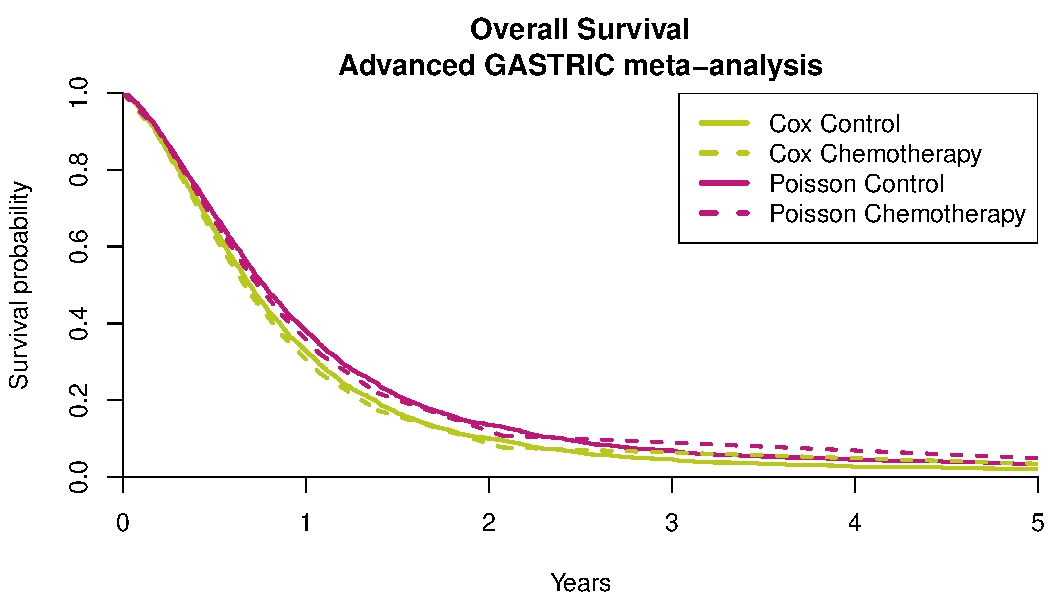
\includegraphics[width=\maxwidth]{figs/figpoissonize-1} \caption{Overall survival curves in the advanced GASTRIC meta-analysis. \textbf{(a)} Comparison between the survival probability obtained using the Breslow estimator in the Cox model (solid lines) and those obtained using the auxiliary Poisson model (dashed lines). \textbf{(b)} Piecewise constant hazard estimated by the auxiliary Poisson model}\label{fig:poissonize}
\end{figure}


\end{knitrout}
The option \inline{add = TRUE} is used to add the curves to the plot
  from the Cox estimates drawn previously.

The treatment effect estimated by the Cox model is
  -0.14 (SE = 
  0.03), 
  and it is -0.14 (SE = 
  0.03)
  when using the auxiliary Poisson model.
\end{document}
